%%% LaTeX Template: Two column article
%%%
%%% Source: http://www.howtotex.com/
%%% Feel free to distribute this template, but please keep to referal to http://www.howtotex.com/ here.
%%% Date: February 2011

%%% Preamble
\documentclass[	DIV=calc,%
							paper=a4,%
							fontsize=12pt,%
							onecolumn]{scrartcl}	 					% KOMA-article class

\usepackage{lipsum}													% Package to create dummy text
\usepackage[brazil]{babel}										% English language/hyphenation
\usepackage[protrusion=true,expansion=true]{microtype}				% Better typography
\usepackage{amsmath,amsfonts,amsthm}					% Math packages
\usepackage[pdftex]{graphicx}									% Enable pdflatex
\usepackage[svgnames]{xcolor}									% Enabling colors by their 'svgnames'
\usepackage[hang, small,labelfont=bf,up,textfont=it,up]{caption}	% Custom captions under/above floats
\usepackage{epstopdf}												% Converts .eps to .pdf
\usepackage{subfig}													% Subfigures
\usepackage{booktabs}												% Nicer tables
\usepackage{fix-cm}													% Custom fontsizes
\usepackage[utf8]{inputenc}
\usepackage[top=2.5cm, bottom=2.5cm, left=2.5cm, right=2.5cm]{geometry}
\usepackage[ddmmyyyy]{datetime}
\addto\captionsenglish{%
	\renewcommand\tablename{Tabela}
	\renewcommand\figurename{Figura}
} 
 

 
%%% Custom sectioning (sectsty package)
\usepackage{sectsty}													% Custom sectioning (see below)
\allsectionsfont{%															% Change font of al section commands
	\usefont{OT1}{phv}{b}{n}%										% bch-b-n: CharterBT-Bold font
	}

\sectionfont{%																% Change font of \section command
	\usefont{OT1}{phv}{b}{n}%										% bch-b-n: CharterBT-Bold font
	}



%%% Headers and footers
\usepackage{fancyhdr}												% Needed to define custom headers/footers
	\pagestyle{fancy}														% Enabling the custom headers/footers
\usepackage{lastpage}	

% Header (empty)
\lhead{}
\chead{}
\rhead{}
% Footer (you may change this to your own needs)

%% ====================================
%% ====================================
%% mude o rodape  do projeto
%% ====================================
%% ====================================

\lfoot{\footnotesize \texttt{Cabeamento estruturado} \textbullet ~Modelo de projeto}


\cfoot{}
\rfoot{\footnotesize página \thepage\ de \pageref{LastPage}}	% "Page 1 of 2"
\renewcommand{\headrulewidth}{0.0pt}
\renewcommand{\footrulewidth}{0.4pt}



%%% Creating an initial of the very first character of the content
\usepackage{lettrine}
\newcommand{\initial}[1]{%
     \lettrine[lines=3,lhang=0.3,nindent=0em]{
     				\color{DarkGoldenrod}
     				{\textsf{#1}}}{}}



%%% Title, author and date metadata
\usepackage{titling}															% For custom titles

\newcommand{\HorRule}{\color{DarkGoldenrod}%			% Creating a horizontal rule
									  	\rule{\linewidth}{1pt}%
										}

\pretitle{\vspace{-30pt} \begin{flushleft} \HorRule 
				\fontsize{40}{40} \usefont{OT1}{phv}{b}{n} \color{DarkRed} \selectfont 
				}

%% ====================================
%% ====================================
%% mude o titulo  do projeto
%% ====================================
%% ====================================

\title{Projeto Cabeamento Estruturado - Empresa Segurança Eletrônica}					% Title of your article goes here

%% ====================================



\posttitle{\par\end{flushleft}\vskip 0.5em}

\preauthor{\begin{flushleft}
					\large \lineskip 0.5em \usefont{OT1}{phv}{b}{sl} \color{DarkRed}}
\author{Anderson Luis de Souza}  	% Author name goes here


\postauthor{\footnotesize \usefont{OT1}{phv}{m}{sl} \color{Black} 
					\\Universidade Tecnológica Federal do Paraná - Câmpus Cornélio Procópio 								% Institution of author
					\par\end{flushleft}\HorRule}

\date{}																				% No date




%%% Begin document
\begin{document}
\maketitle
\thispagestyle{fancy} 	
\thispagestyle{empty}		% Enabling the custom headers/footers for the first page 
% The first character should be within \initial{}




%% ====================================
%% ====================================
%% mude o resumo  do projeto
%% ====================================
%% ====================================

\initial{E}\textbf{ste projeto trata-se de uma reestruturação de uma empresa de segurança eletrônica. Tal empresa possui uma central de monitoramento com até 6 atendentes simultâneos, utilizando estrutura IP para desktops e telefones. Além da sala de monitoramento, possui setores administrativo, comercial, diretoria, entre outros. 
Será feito um levantamento da estrutura física do cliente, a fim de obter o cenário atual da empresa, para determinar quais as mudanças serão implantadas.
Será elaborado a planta lógica, levantamento de equipamentos passivos, de custos, e também um plano de certificação.
A finalidade desta reestruturação é a organização e viabilizar o crescimento da rede, tornando as manutenções mais rápidas.}


%% ====================================
\begin{figure}
	\centering
	
\includegraphics{utfpr}
\end{figure}

\vspace{2cm}
\centerline{\textit{\textbf{\today}}}

\clearpage
    \renewcommand*\listfigurename{Lista de figuras}
\listoffigures

\renewcommand*\listtablename{Lista de tabelas}
\listoftables




\clearpage
\renewcommand{\contentsname}{Sumário}
\tableofcontents
\clearpage

%% ====================================
%% ====================================
%% Inicio do texto
%% ====================================
%% ====================================
\section{Introdução}
Com foco principal em viabilizar a expansão da empresa, o setor de ti da empresa, propõe uma reestruturação e planejamento da rede de computadores.

A empresa presta serviços de segurança eletrônica e portaria remota, em empresas e condomínios. Atualmente possui cerca de 25 colaboradores que revezam em escalas. O principal setor da empresa é a base de monitoramento, no qual hoje possui 6 estações de atendimentos simultâneas. A empresa também é dividida em outros setores, sendo, financeiro, comercial, recepção, diretoria, ti e operacional.

Como meta de crescimento, a empresa deseja até o ano de 2021 possuir 10 estações de atendimento, além da expansão dos outros setores.

\subsection{Benefícios}
Neste projeto, o cliente contara com diversos benefícios, como:

\begin{itemize}
	\item Viabilizar a expansão dos negócios da empresa
	\item Facilitar manutenções e novas implantações
	\item Organização e identificação dos pontos de rede
	\item Padronização e certificação
\end{itemize}

\subsection{Organizações Envolvidas}
Por se tratar de uma reestruturação da empresa, todos os setores estarão envolvidos, porém, não será distribuído funções para estes setores.
O setor de TI estará diretamente envolvido com esta reestruturação, sendo este o principal contato para tais alterações.

\section{Estado atual}
Para fins informativos, o estado atual da rede é:

\begin{itemize}
	\item 2 Switch de 24 Portas não gerenciado
	\item 1 Switch de 16 Portas não gerenciado
	\item 3 Patch panel 24 portas Cat5e
	\item Cabeamento Cat5e
	\item 1 RouterBoard Mikrotik 3010
	\item 3 Servidores Torre fixados no rack
	\item 1 Servidor Voip
	\item 16 Estações de trabalho Desktop
	\item 20 Telefones IP
	\item 1 Internet 200MB/200MB GPOM
	\item 10 Links de dados SLDD 4MB FULL
	\item Nobreak NHS 2600 VA + Módulo de Bateria
	\item Gerador Toyama 7 Kva
\end{itemize}

\section{Requisitos}
Para a implantação deste projeto, o cliente deverá providencial alguns requisitos, como tubulação, móveis, além dos itens descritos na tabela 1.

\input{tabRequisitos}

\section{Usuários e Aplicativos}

Atualmente na empresa trabalha-se em horários de pico, no máximo 14 colaboradores simultâneos.

Até 2021 a empresa espera ter cerca de 22 colaboradores simultâneos, divididos entre os diversos setores da empresa.

Os usuários internos utilizam do sistema ERP da empresa, e raramente precisam utilizar da navegação na internet, salvo setor comercial e TI. 
Os colaboradores da base de monitoramento, utilizam de sistema de monitoramento de eventos e câmeras.

Além destes descritos, todas as estações contam com Microsoft Windows 10 Pro, Microsoft Office 2016. Em nível de servidor, estes possuem Microsoft Windows Server 2016 e SQL Server. Em nível de rede, somente o router OS da Mikrotik.

A tabela 2, mostra os perfis de usuários, assim como os aplicativos mais usados por cada um destes.

\begin{table}[h!] % coloque h! para forcar a posicao
	\centering
	\caption{Tabela de Perfil Usuários}
	\label{TabPerfilUsuarios} %com este label vc faz referencia no texto
\begin{tabular}{|c|l|}
	\hline
	\textbf{Perfil} & \multicolumn{1}{c|}{\textbf{Aplicativos Utilizados}}                \\ \hline
	TI              & Windows 10 pro, Windows Server, SQL Server, Office, Router OS, Voip \\ \hline
	Monitoramento   & Windown 10 pro, Office 2016, ERP, Sistema Monitoramento, Voip       \\ \hline
	Comercial       & Windown 10 pro, Office 2016, ERP, Google Chrome, Voip               \\ \hline
	Financeiro      & Windown 10 pro, Office 2016, ERP, Internet Banking, Voip            \\ \hline
	Diretoria       & Windown 10 pro, Office 2016, ERP, Google Chrome, Voip               \\ \hline
	Recepção        & Windown 10 pro, Office 2016, ERP, Voip                              \\ \hline
	Operacional     & Windown 10 pro, Office 2016, ERP, Voip                              \\ \hline
\end{tabular}
\end{table}

\section{Estrutura predial existente}

A figura 1, observa-se a planta física da empresa.

\begin{figure}[h!]
	\centering
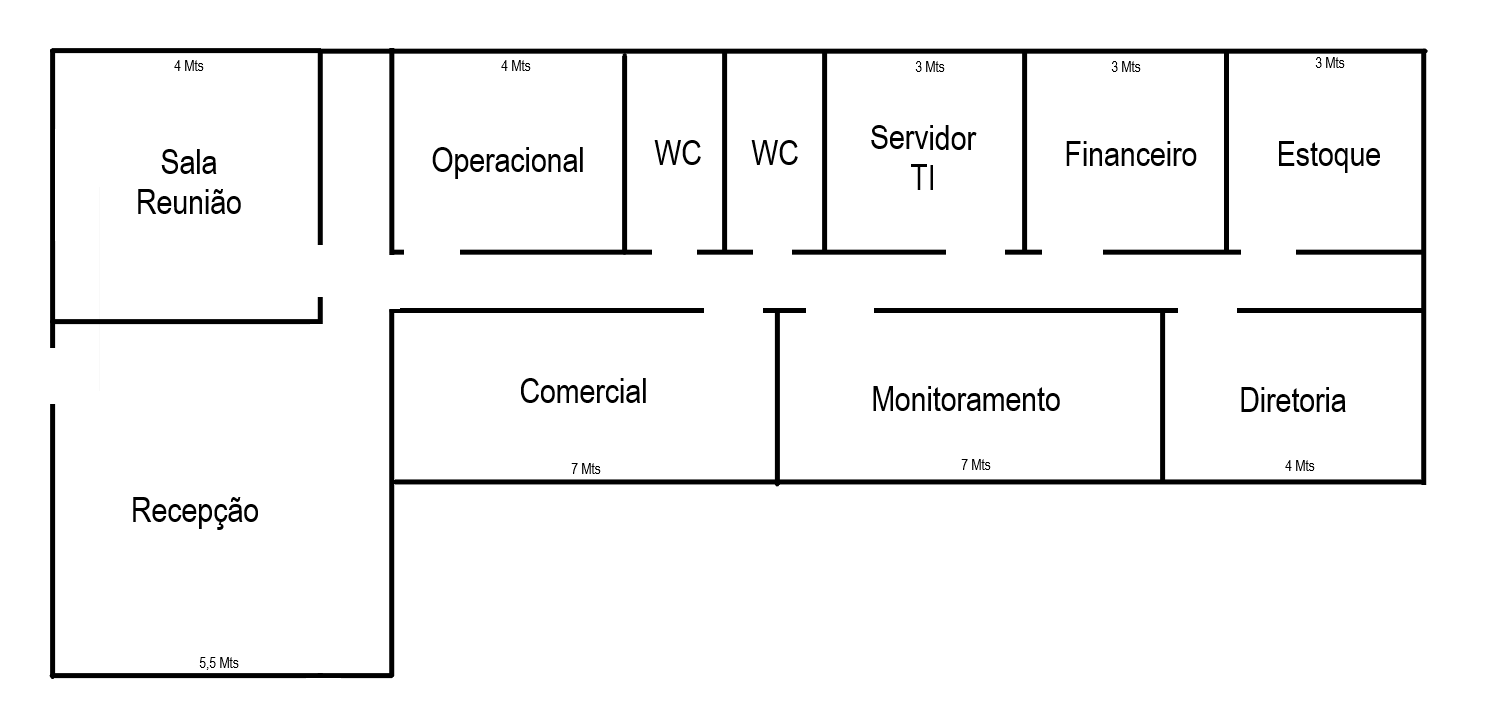
\includegraphics[width=\textwidth]{PlantaEmpresa}
	\caption{Planta Física da Empresa}
	\label{Planta Empresa}
\end{figure}

Nesta planta, observa-se que a distancia entre as salas e o servidor é relativamente pequena, sendo assim, todo o cabeamento ficará abaixo de 100 Mts, não sendo necessário repetidores entre os setores.

Também se observa que as salas são pequenas, possibilitando que sejam implantados cerca de 3 computadores por sala, exceto monitoramento e comercial, que podem ser alocados até 10 computadores cada.

\section{Planta Lógica - Elementos estruturados}

\subsection{Estado atual}

Na Figura 2, se observa a planta lógica atual da empresa, no qual utiliza da topologia estrela, concentrando toda a rede nos switch da sala do servidor.

\begin{figure}[h!]
	\centering
	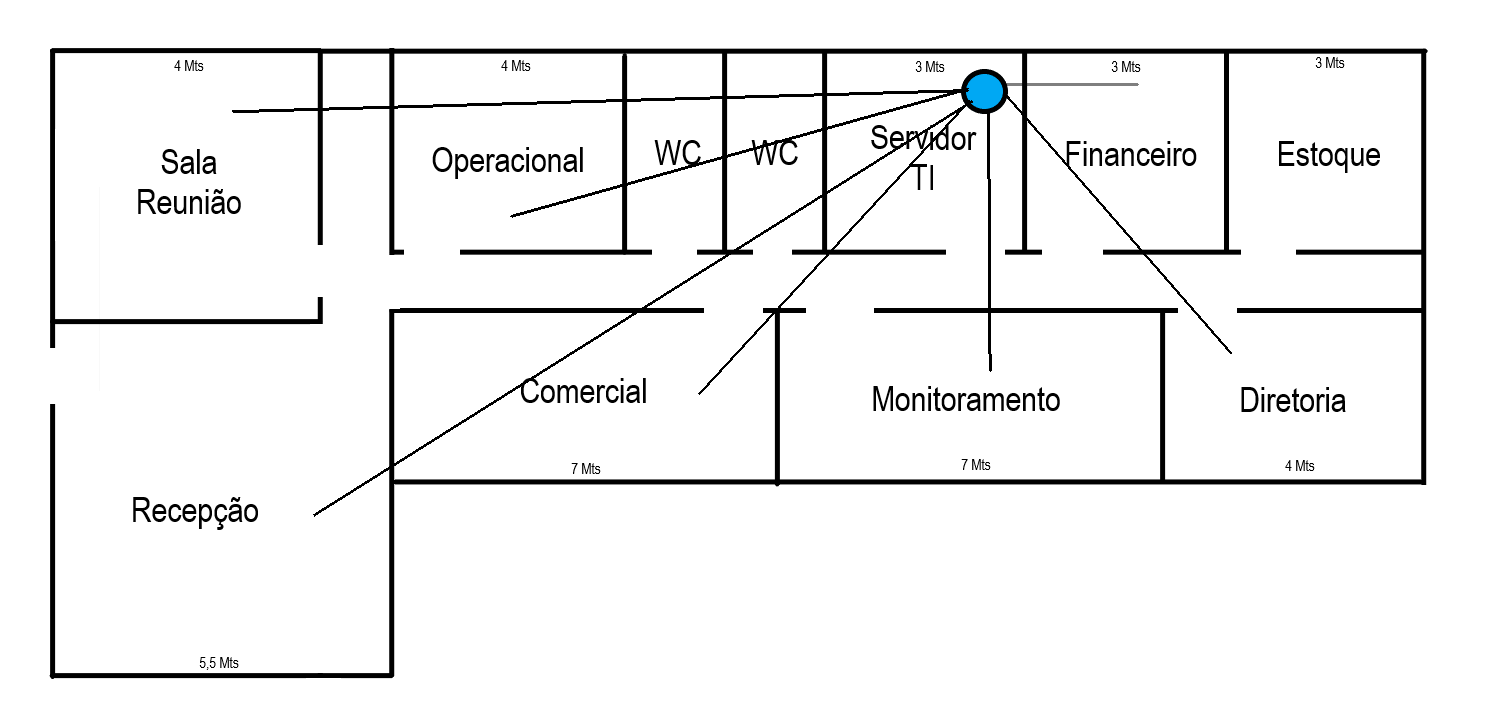
\includegraphics[width=\textwidth]{PlantaLogicaAtual}
	\caption{Planta Lógica Atual da Empresa}
	\label{Planta Lógica Atual}
\end{figure}


\subsection{Topologia}
Proposta futura, proposta após implantação.
Deve conter o diagrama da rede. Atente-se a redundância  e ligações truncadas.
Deve explicar todos termos e componentes utilizados nestas plantas. Por exemplo: entrance facility, work area, horizontal cabling, etc..

Todos os elementos das figuras devem ser explicados. 
Crie esboço da configuração dos racks e brackets. Explique cada um dos componentes. Você pode criar uma tabela contendo figuras dentro, ou criar uma tabela e incluí-la como imagem. Por exemplo, verifique a tabela \ref{tab1}.

\subsection{Encaminhamento}
Será necessário para a execução do projeto, a instalação de eletrodutos galvanizados e eletro calhas, para acomodar os fios. A quantidade de materiais é detalhado na tabela a seguir.

\begin{table}[h!] % coloque h! para forcar a posicao
	\centering
	\caption{Tabela de Encaminhamentos}
	\label{tabEncaminhamento} %com este label vc faz referencia no texto
\begin{tabular}{|c|l|l|}
\hline
\textbf{Quantidade} & \multicolumn{1}{c|}{\textbf{Material}} & \multicolumn{1}{c|}{\textbf{Tamanho}} \\ \hline
15                  & Eletroduto Galvanizado                 & 2 Pol                                 \\ \hline
45                  & Abraçadeiras com Cunha                 & 2 Pol                                 \\ \hline
10                  & Emenda                                 & 2 Pol                                 \\ \hline
15                  & Curva em L                             & 2 Pol                                 \\ \hline
15                  & Caixa Condulete X                      & 2 Pol                                 \\ \hline
10                  & Eletrocalha                            & 120 mm                                \\ \hline
20                  & Emenda Eletrocalha                     & 120 mm                                \\ \hline
30                  & Suporte Eletrocalha                    & 30 Cm                                 \\ \hline
5                   & Curva em L Eletrocalha                 & 120 mm                                \\ \hline
100                 & Parafuso e Porca                       &                                       \\ \hline
\end{tabular}
\end{table}

\subsection{Memorial descritivo}

Relacione todos os equipamentos passivos que serão utilizados, tipo, fabricante, quantidade.

\subsection{Identificação dos cabos}
Explique como os cabos serão identificados em seu projeto. Coloque uma relação dos cabos instalados e identificados.

\section{Implantação}
Estabeleça um cronograma de implantação:
Remoção de equipamentos existentes (destino para descarte), instalação dos condutores, instalação dos cabos, 
identificação dos cabos, montagem dos racks, certificação, etc... Crie atividades e estabeleça o tempo de execução. Se for um projeto real, indique também quais os responsáveis pela execução do projeto e de cada uma das etapas.

Defina marcas (e padrões) e fornecedores se for o caso. Atenção a contratados e subcontratados para a realização das atividades. Estabeleça a responsabilidade de execução da atividade e também da validação dela.

Utilize algum software para gerear o cronograma. Excel,etc. O fundamental é dividir em etapas, descrever e estimar o tempo de cada uma delas.

Segue uma relação de ferramentas:
http://asana.com/, 
https://trello.com/, 
http://www.ganttproject.biz/, 
http://www.orangescrum.org/. 

\section{Plano de certificação}
Quais seriam as etapas para a certificação? 
Quais os locais e horários para execução da certificação na rede? Toda rede será certificada?
Como os testes seriam executados?
Quais relatórios de certificação serão (ou deveriam ser) entregues? 

\section{Plano de manutenção}

Revisões periódicas na rede, emissão de certificados para novos pontos.

\subsection{Plano de expansão}
Existe um plano de expansão? Quantos novos pontos poderão ser acrecidos na rede, antes de migração de equipamentos na camada 2? Se houver expansão, quais equipamentos deverão ser direcionados para as estremidades da rede? 

\section{Risco}
Enumerar e explicar os riscos do projeto.

\section{Orçamento}
Crie uma relação de orçamentos baseado na seções anteriores.

\section{Recomendações}
Observações e recomendações para o cliente.

\section{Referências bibliográficas}
Utilize o mendley, o jabref ou diretamente o bibtex para gerenciar suas referências biliográficas. As referências são criadas automaticamente de acordo com o uso no texto.

Exemplo: Redes de computadores, segundo \cite{t2013} é considerada..... Já \cite{kurose2010} apresenta uma versão...

Analisando os pressupostos de \cite{ref3} e \cite{ref4} concluimos que....


\renewcommand\refname{} %%Referências bibliográficas}  
\bibliographystyle{ieeetr}
\bibliography{referencias}  

%% ***********************************************************************
%% === remover daqui =====================================================
%% ***********************************************************************
=================================================
\section{Elementos textuais - Alguns exemplos}

Esta seção apresenta exemplos de elementos textuais. \textbf{Remova-a da versão final do texto}.


\subsection{Colocar elementos em itens}

Texto antes da lista

\begin{itemize}
	\item First item in a list 
	\item Second item in a list 
	\item Third item in a list
\end{itemize}

\subsubsection{Uma subseção de terceiro nivel}

Exemplo de uma subseção

\subsection{Tabelas}

Utilize o site http://www.tablesgenerator.com/ para elaborar as tabelas de seu trabalho.
Para adicionar uma tabela utilize: a tag input, passando o arquivo da tabela como parametro

\begin{table}[h!] % coloque h! para forcar a posicao
\centering
\caption{Modifique a legenda e crie um label}
\label{tab2} %com este label vc faz referencia no texto
\begin{tabular}{|l|l|l|l|l|}
\hline
\multicolumn{1}{|c|}{\textbf{Este é um exemplo de tabela}} & \multicolumn{2}{c|}{\textbf{C1}} & \multicolumn{2}{c|}{\textbf{C2}} \\ \hline
Você pode criar a tabela no excel                          & 1              & 2               & 3               & 4              \\ \hline
Exportar para CSV                                          & 5              & 6               & 7               & 8              \\ \hline
E importar no Table Generator                              & 9              & 10              &                 &                \\ \hline
\multicolumn{5}{|c|}{\textit{Gere o tex, e adicione em seu arquivo}}                                                             \\ \hline
\end{tabular}
\end{table}

Dentro do arquivo você deve definir o label e pode utilizá-lo para referenciar. Exemplo:
Na tab \ref{tab2} temos a relação de ....


Você também pode modificar a tabela manualmente, incluindo, por exemplo h! dentro de sua definição. Veja no exemplo tab2.tex

\subsection{Figuras}

As figuras podem ser no formato PDF, JPG, PNG. Você pode referenciá-las da mesma maneira que tabelas. Exemplo: A figura \ref{fig1} apresenta.....

Não se preocupe o local em que a figura será renderizada em seu texto. Preocupe-se em criar referência para ela, ou seja, toda figura e tabela deve conter pelo menos uma referência no texto.

\begin{figure}
\centering
\includegraphics[width=\textwidth]{fig1}
\caption{Exemplo de figura com escala horizontal}
\label{fig1}
\end{figure}


\begin{figure}
	\centering
	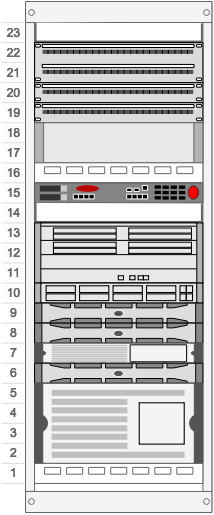
\includegraphics[]{fig2}
	\caption{Exemplo de figura sem escala}
	\label{fig2}
\end{figure}

Você pode rotacionar figuras também. Para isso utilize o parâmetro angle=-90. Repare que a escala da figura foi modificada pelo parametro height. Você também pode utilizar scale

\begin{figure}
	\centering
	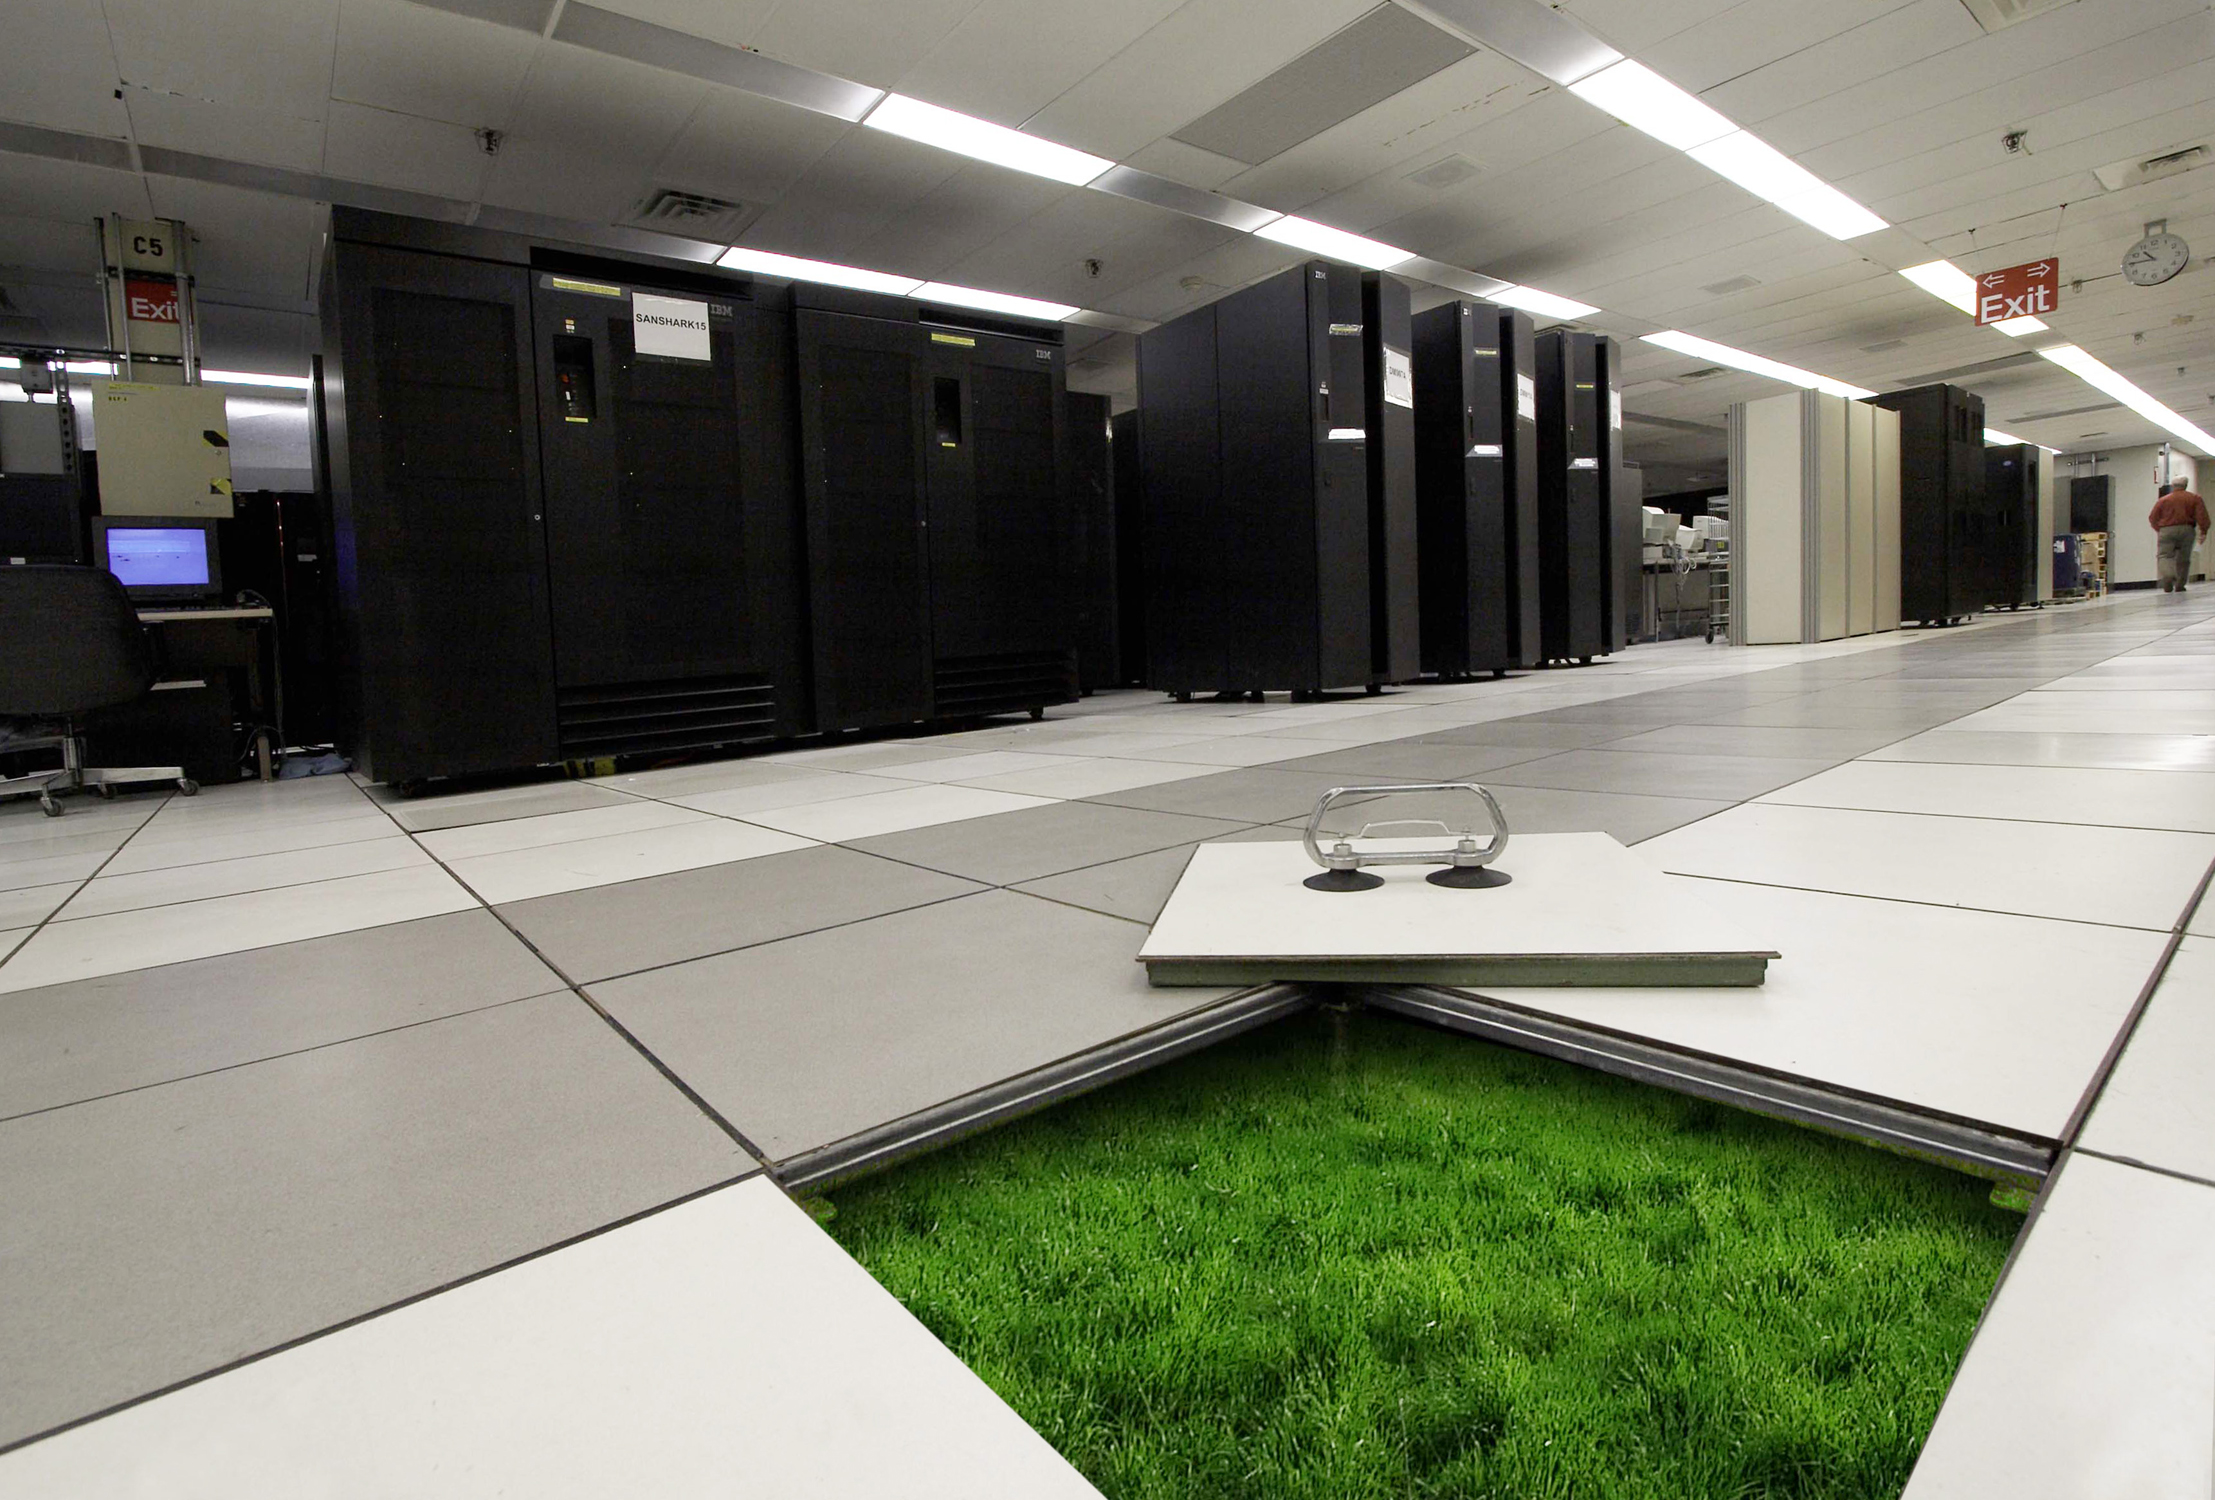
\includegraphics[height=\textwidth,angle=-90]{fig3}
	\caption{Exemplo de figura rotacionada}
	\label{fig3}
\end{figure}

Você também pode inserir páginas de outro tamanho em seu texto. Isto irá ajudar a inserir imagens maiores, como as desenvolvidas em CAD. Segue um exemplo na figura \ref{fig4} e figura \ref{fig5}.


%inicio dos comandos para criar uma nova pagina A3
\clearpage
\KOMAoptions{paper=a3, pagesize}
\recalctypearea

\begin{figure}
	\centering
	\makebox[\textwidth][c]{
		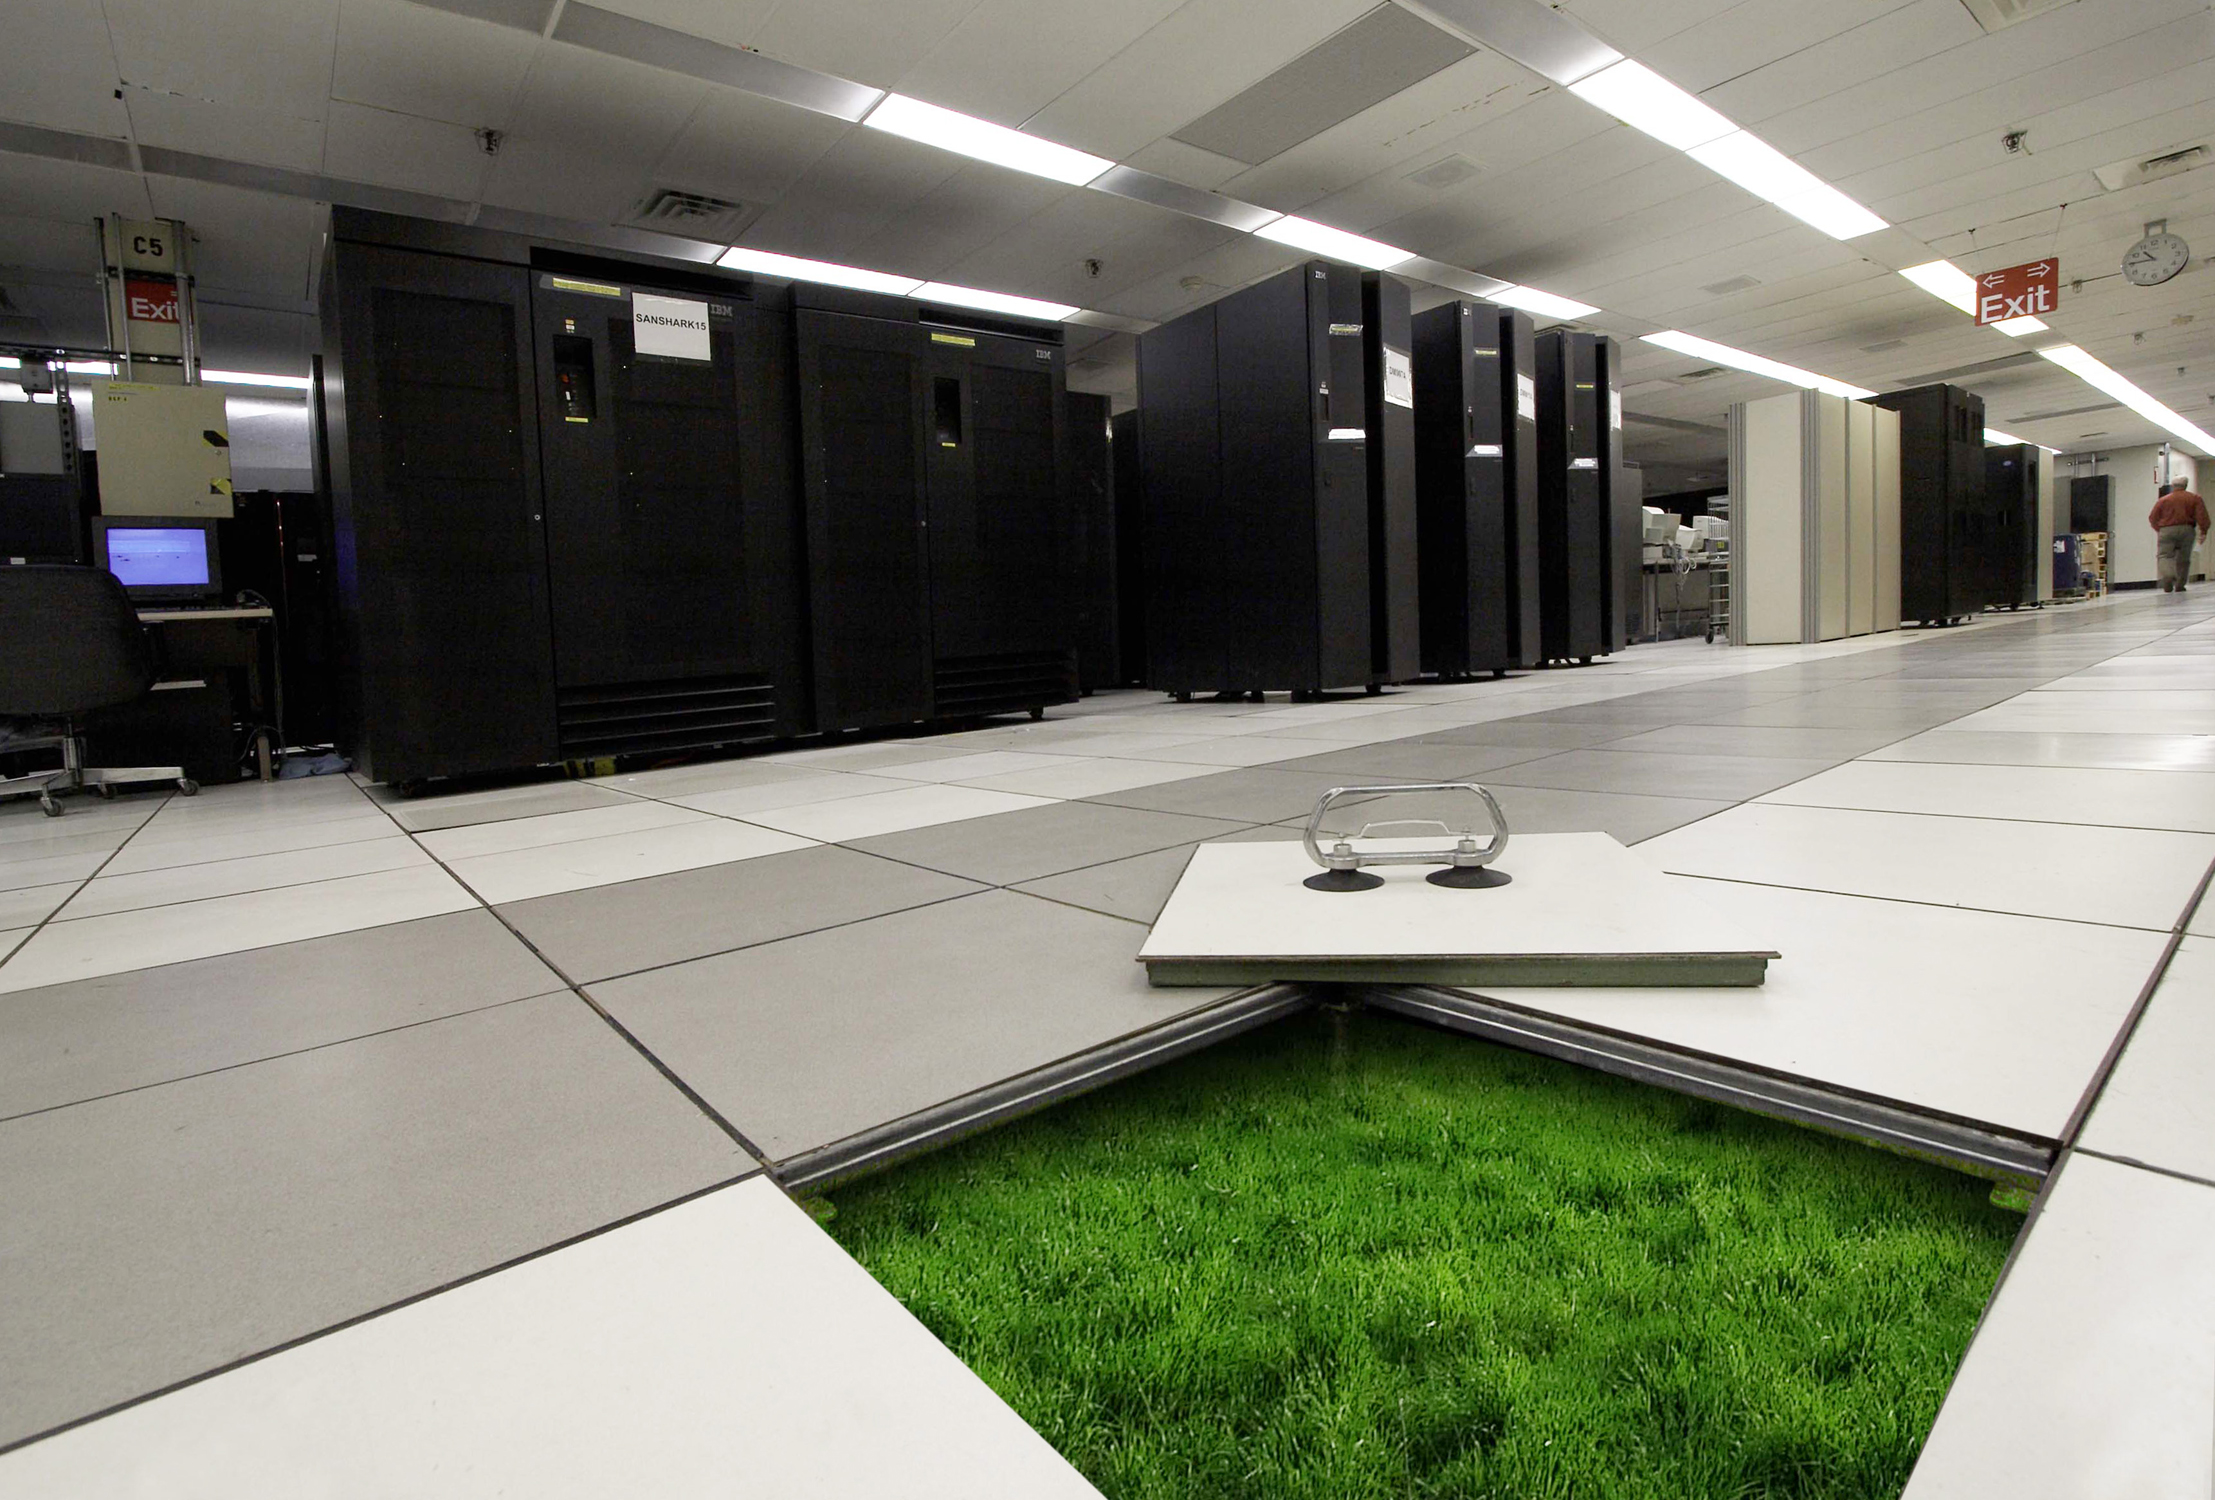
\includegraphics[height=\textheight]{fig3}}
	\caption{Exemplo de figura inserida em uma página A3}
	\label{fig4}
\end{figure}

%Retornar ao formato A4
\clearpage
\KOMAoptions{paper=a4, pagesize}
\recalctypearea
%-- reinicio em A4 


%inicio dos comandos para criar uma nova pagina A3 horizontal
\clearpage
\KOMAoptions{paper=a3, paper=landscape, DIV=20}
\recalctypearea

	
\begin{figure}
%	\centering
	\noindent\makebox[\textwidth][c]{
		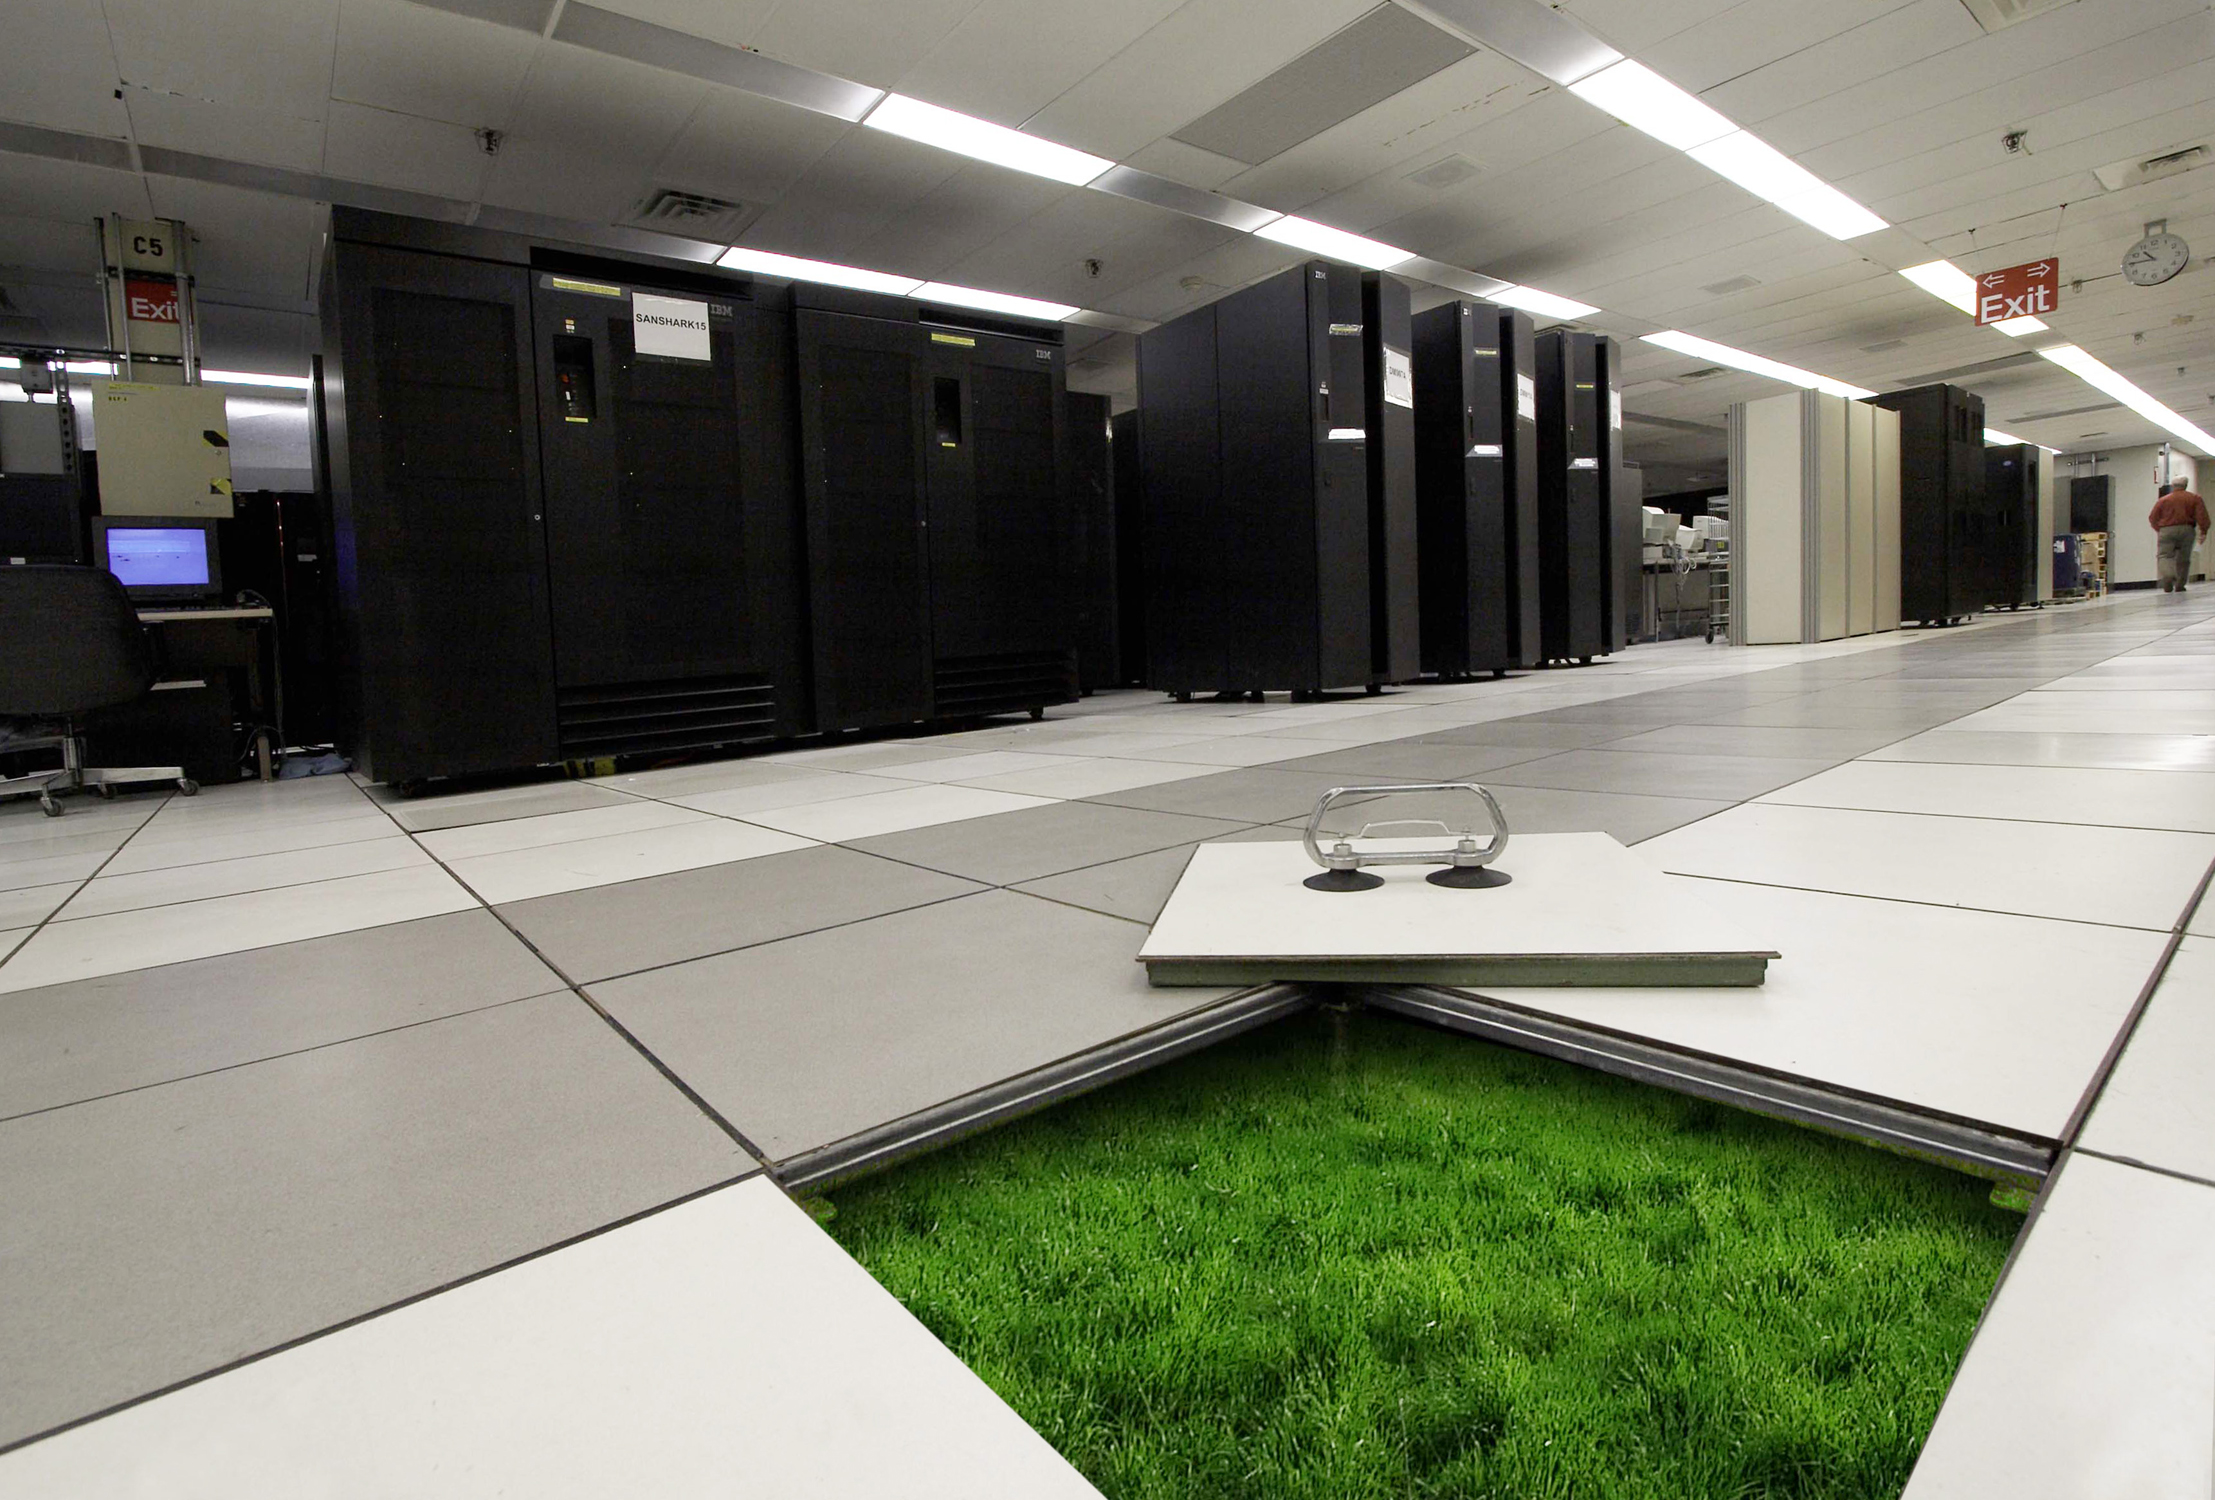
\includegraphics[width=\textwidth]{fig3}
	}
	\caption{Exemplo de figura inserida em uma página A3 no formato horizontal}
	\label{fig5}
\end{figure}

%Retornar ao formato A4
\clearpage
\KOMAoptions{paper=a4, paper=portrait, DIV=15}
\recalctypearea
%-- reinicio em A4 


\subsubsection{Resumo gráfico}

Você pode optar por fazer um resumo no formato de mapa mental/conceitual. 
Aqui foi utilizado o site https://app.mindmup.com para gerar o mapa.

Para utilizar o resumo gráfico, remova o texto da seção resumo (linha 137) e inclua o código para inserir a figura, conforme figura \ref{fig6}

\begin{figure}[h]
	\centering
	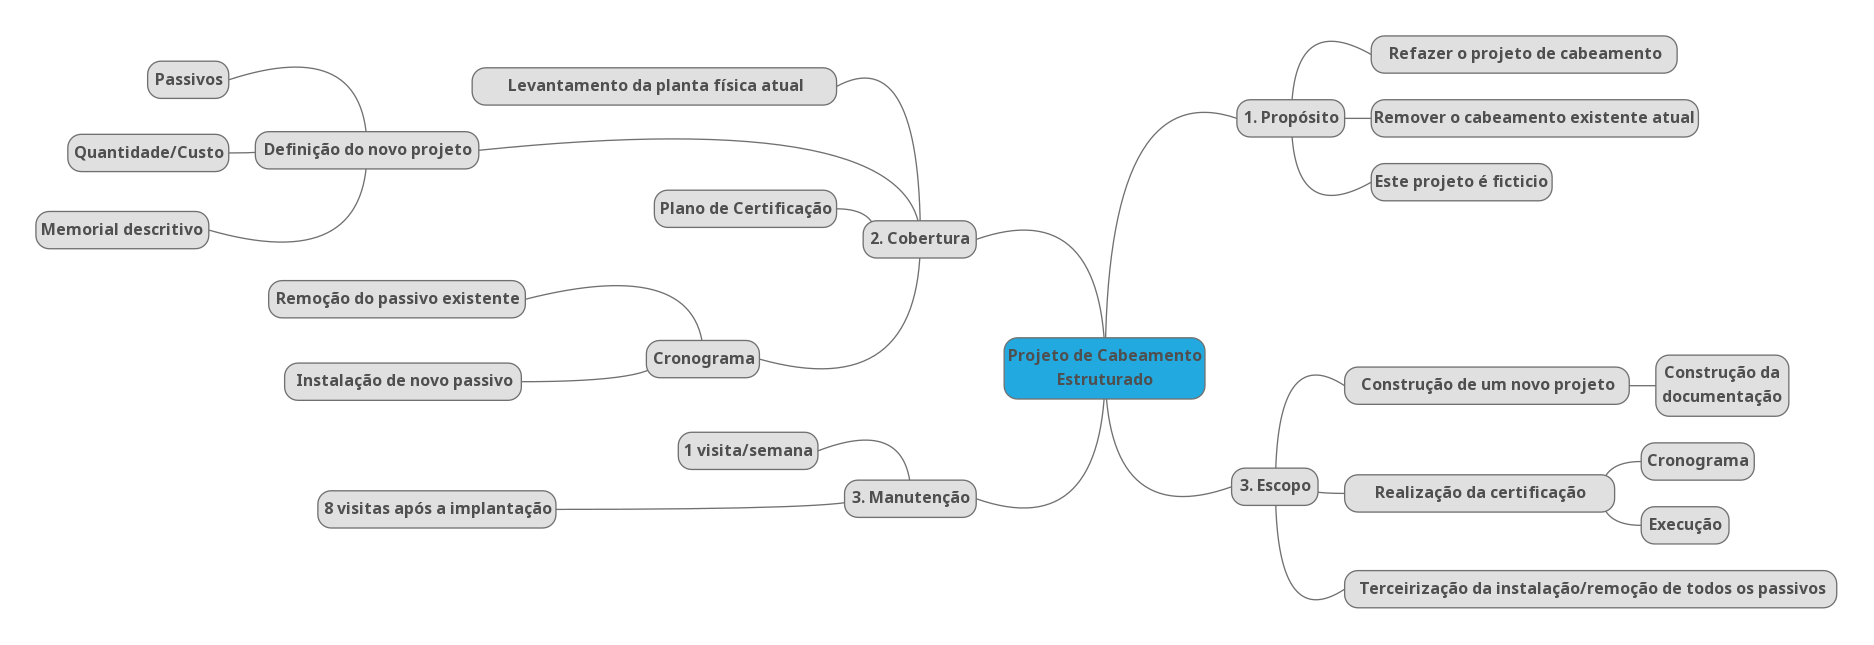
\includegraphics[width=\textwidth,height=5cm,keepaspectratio]{fig4}
	\caption{Exemplo de resumo gráfico}
	\label{fig6}	
\end{figure}

%% ***********************************************************************
%% === ate aqui    =====  ================================================
%% ***********************************************************************

\end{document}